% Chapter 1

\chapter{Introduction}

\label{chap:introduction} 

\graphicspath{{Figures/Introduction}}

Programming languages are the media through which we communicate our ideas with machines, be it mathematical formulae or video games. Like human language, programming languages consist of words, grammar, and meaning. Unlike conversing with humans, machines tolerate very little ambiguity and are not skillful at navigating confusion. Furthermore, sometimes inconsistencies glossed over by humans can be indicative of bigger oversights - for example, mismatched types can be indicative of an ill-defined mapping. In this chapter, we inspect two spectrums of programming language design: their typing disciplines and the paradigms in which they reside. Through this, we hope to illustrate a common patern in programming: the more certainty we get knowing our program runs correctly, the more we are bothered with conforming to rules and checks. And when these rules and checks are violated, we meet the anguish of the compiler in arcane jargon, sometimes all in uppercase letters. My interventions -- most notebly, Chameleon, Goanna, and GeckoGraph -- aim to replace the terse and static error messages with a clear diagnosis system, assisted by the interactive user interface, to provide programmers with clarity, intuitiveness, and resolution. Clarity means providing succinct and accurate explanation of errors. Intuitiveness measn presenting the error diagnosis in interfaces that are easy to learn, understand, and use. These systems aim to  expose all internal required to make informed decisions, give programmers better changes at solving erros as well as further their understanding of the languages they are using.


\section{From types to program correctness}

In programming language theory and practice, typing is a widely adopted program validation method where types of expressions are checked against their usage. In the early history of programming, types were used to inform the compiler how much memory needs to be allocated for each value. Now, type systems are much more powerful; programmers can express complex ideas, like communication protocols and concurrency characteristics. Conventionally, the discipline of typing is identified by the existence of a compile-time checking stage. A programming language is said to be statically typed if checks are performed before a program is executed.  On the other hand, dynamically typed languages (colloquially called dynamic languages) will not complain about type mismatch prior to the program being run, and they do not facilitate describing the types (Fig. \ref{fig:typed-vs-untyped}). In dynamic languages, expressions like \texttt{4 + "2"} will result in a runtime error; some languages try to coerce the data on behalf of the programmer and produce results like ``42''. Statically-typed languages have a long history and are extremely popular, with examples among both the earliest of programming languages (such as FORTRAN and ALGOL, \cite{Backus1978-xt}) and the most widely-used languages across all platforms  (such as C and its derivatives, including Java and C\#, \cite{Ritchie1978-pa}). Static typing is also a core feature of the most advanced and renowned academic languages (such as ML, Haskell, and their derivatives, such as OCaML and Agda, respectively, \cite{Hudak2007-kn}). In practice, statically typed programming languages offer many advantages. Type declarations and annotations add important contextual information about the expected use of variables and expressions. This additional context allows early error detection but also enhances code readability and promotes maintainability, especially in large collaborative projects. The explicit encapsulation of type information in code also creates opportunities for improved tooling through intelligent compiler services and IDE (interactive development environment) support. Additionally, static typing enhances code documentation by providing clear contracts between library authors and users and, more generally, enhancing code reusability.


In comparison, dynamic typing provides many appealing benefits and has an equal, if not stronger, influence in the computing world. In dynamically-typed languages, a variable can hold different types of values because the type is checked during runtime. This provides more flexibility than static typing since a function can be used to process different types of input values without any special semantics. However, it also means that errors such as trying to subtract a string from a number can be detected only when the code has been run, leading to potentially dire consequences. Programming languages in the Lisp family, such as Common Lisp and Scheme, were designed to benefit from the flexibility of dynamic typing. In Lisp languages, a common design pattern is that functions take dynamic input that can assume various forms (atom, lists, s-expressions), and different code is executed based on inspecting the input value at runtime. Another benefit of dynamic languages is that they are easier to learn. Programmers need not worry about declaring and conforming to types at all, and they can jump directly into computation. In modern-day computing, prolific languages like JavasScript and Python are dynamic, which is believed to contribute to their immense popularity thanks to the lower barrier of entry.

\begin{figure}[hbt]
  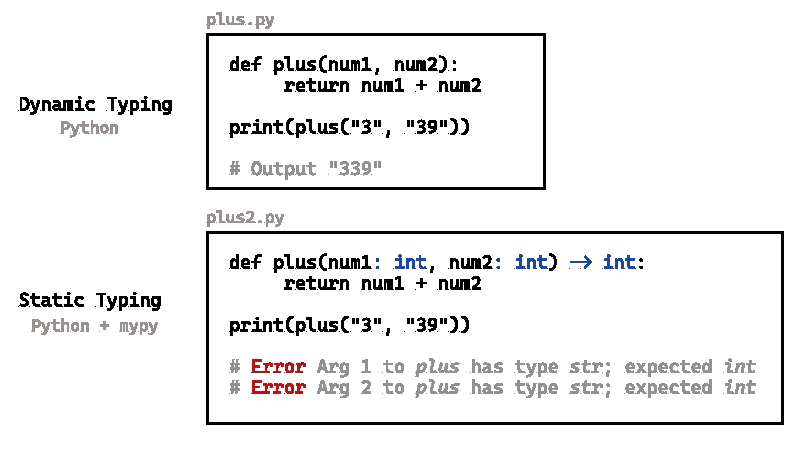
\includegraphics[width=\linewidth]{TypedVsUntyped.pdf}
  \caption{
    \label{fig:typed-vs-untyped}
   The same program is dynamically typed in Python (Top) and with Python + mypy -- a static typing tool for Python (Bottom).
    }
\end{figure}

It comes as no surprise that large amounts of work were dedicated to deciding which one of the two typing disciplines is superior.   Unfortunately, no universal agreements can be drawn from these studies.  Some studeis support the \cite{Ray2017-gq, Kleinschmager2012-bg, Mayer2012-qc, Gao2017-xn}.  Software qualities \cite{Ray2017-gq, Gao2017-xn}, ease of maintainability \cite{Kleinschmager2012-bg}, speed of fixing errors \cite{Prechelt1998-pd}, speed of implementing features \cite{Prechelt2000-bf, Mayer2012-qc}, ease to understand \cite{Endrikat2014-uz}. Very rarely, study \cite{Hudak1994-ex} showed significant result, indicating `` Haskell prototype took significantly less time to develop and was
considerably more concise and easier to understand ".  However, this study needs to be taken with a grain of salt, as the author is one of the  original creater of Haskell language and wrote the Haskell prototpye in the study. Nevertheless, the conventional wisdom on this issue is that dynamically type languages are often more beginner-friendly, better fit for rapid-prototyping; statically type languages show more stengths in larger progjects, easier on onging change requets, producing more solid and robust code base thanks to its soundness features. 

\section{Functional Programming}
Of course, static typing is not the only technique that embraces rigor and formalism. \textbf{Functional languages}, inspired by Alonzo Church's lambda calculus \cite{Church1985-bx} in the 1930s, promotes the idea of using functions as the fundamental building blocks of programming and developing abstractions by composing functions. 
So-called `pure' functional programming languages adopt additional rigor from mathematics, such as immutable values (values can not be modified once declared) and referential transparency (functions always produce the same output when given the same input).  Like static typing, functional language concepts help programmers avoid certain undesired behaviors. For instance, because of the removal of mutable pointers and shared memory,  misaligned pointers and race conditions are essentially eliminated. Thus, programs written in these languages can be safely tested and reasoned about, and it takes away the fear that program behavior can be disrupted by external uncertainties, such as network connections or even dates. 

Functional programming has been advocated as an ideal introductory programming language. Its advocates argue that it promotes mathematical thinking and enforces strict programming discipline (such as separating data and transformation). 

\begin{figure}[hbt]
  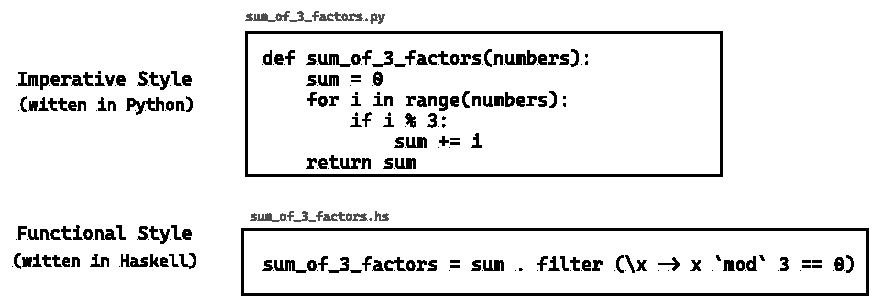
\includegraphics[width=\linewidth]{ImperativeFunctional}
  \caption{
    \label{fig:imperative-vs-functional}
   The same task of summing the factors of 3 in the given numbers, written in imperative style (Top) and functional style (Bottom).
    }
\end{figure}

Other paradigms of programming include object-oriented (in which programs are organized by objects, within which data and behavior co-habit) and procedural programming (inwhich programs are written by specifying a series of steps). In today's programming industry, these paradigms are still more popular than functional languages. The traditional long-serving languages, such as C (procedural) and Java (Object-oriented), are more commercially successful than any functional languages. Thus, they are attracting new software projects that depend on their time-tested codebase, vast 3rd party library support, and familiarity with tools. Additionally, they often are able to provide better performance by offering a set of low-level programming semantics that are close to the hardware. In C, pointers, locks, and manual memory allocation are common concepts that encourage fast memory sharing and efficient concurrency. Lastly, the strictness in functional programming languages may raise the barrier to entry for beginners. For example, in many pure function languages, printing to the terminal window, generally considered a basic technique to observe the execution of the program, requires programmers to understand deep concepts like monad and side effects.  


\section{Statically-Typed Functional Languages, The Best Of Both Worlds}
Combining the disciplines described above, \textbf{statically-typed functional languages} employ both static typing and the principles of functional programming. The most common statically-typed functional languages include Haskell,  ML (with the OCaml dialect being the most popular among the family of ML languages), and F\#. 
Of these, Haskell is the only ``pure'' functional language - with all variables being immutable by default.
Descendents of Haskell, like Idris and Agda, include more advanced type-level features like dependent type and session type, allowing programmers to express extremely granular checks of potential software behavior before running the program. These languages often provide the strongest level of programming safety. It is often advertised that programs in these languages will be error-free if the source code passes the compiling stage, indicating that compilers are able to weed out a large number of programming errors. These safety properties allow statically-typed functional languages to be used as proof assistants or formal verification tools. They prove the correctness (or incorrectness) of many systems, from web public key infrastructure \cite{Bhargavan2021-no} to microcontrollers used in space programs \cite{Mokhov2019-zj}. Despite these safety benefits, these languages' presence in the mainstream programming world remains underwhelming. This lack of popularity is often attributed to higher barriers to entry, unfamiliarity, and unforgiving type errors.

\section{Symptoms of Bad Type Errors}
\ref{sec:symptoms}
 The compiler is the medium through which programmers transform human intention into machine instructions. When encountering errors, compilers often act like ancient oracles, revealing to programmers obscure messages that often lead to huge confusion and a wrong course of action. Many studies have investigated the ineffectiveness of compiler error messages \cite{Barik2017-gy, Becker2019-cs, Becker2016-kc}.  To illustrate the point, we use the Haskell language and its most popular compiler, the Glasgow Haskell Compiler (GHC), as our development testbed and focus our attention on improving upon the state of GHC's type error communications. However, it needs to be clarified that the issues with compilation errors underpinning the examples we consider are typical of statically-typed programming language compilers. We now detail a variety of symptoms of bad type error messages.



 \subsection{Bias in Type Errors} 
 \label{subsec:bias}
 Bias in type error is when a type error can be caused by any one of multiple sources, but the type error only reports one of them. This limitation, known as left-to-right bias, has often been criticized \cite{McAdam2002-vb, Lee1998-fx, Chen2014-ev} as a drawback of compiler error messages. Left-to-right bias is a fundamental limitation of the traditional type-checking algorithm, which we will revisit in greater detail in Chapter \ref{chap:haskell-type-checking}. In the example in Fig. \ref{fig:type-error-example}, it is more likely that the programmer intends to compute the sum of the two input numbers using the addition function \texttt{+} rather than concatenating the two inputs using the concatenation function \texttt{++}. However, the type error shows only one error, suggesting that the function \texttt{addTwoNumbers} is given the wrong type of argument. 

 \begin{figure}[hbt]
  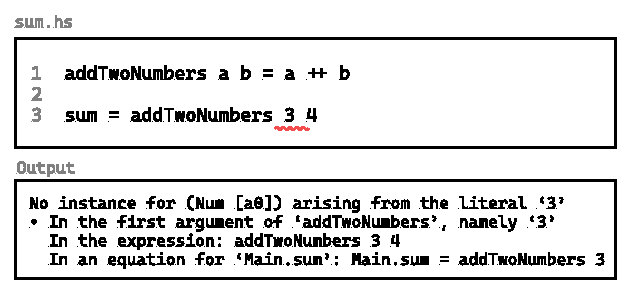
\includegraphics[width=\linewidth]{TypeErrorExample}
  \caption{
    \label{fig:type-error-example}
  In this example, the programmer likely misused the concatenation function \texttt{++} rather than addition \texttt{+} on line 1. However, the compiler will report that the error is the application of the integer literal \texttt{3}.
    }
\end{figure}


\subsection{Type Error Suggests Incomplete Cause}
\label{subsec:imcomplete}

Type error messages often show an incomplete cause, meaning that fixing the highlighted location alone is not sufficient to resolve the type error. In the example in \ref{fig:type-error-example-2}, similar to the previous example with the only change being the name of the function, suppose that the programmer intended to write the function to concatenate two lists but apply the function with 2 integer values. However, in the type error, only the first argument is reported as an offending code; the second argument is spared. The programmer changing the literal \texttt{3} to \texttt{[3]} is not enough to make the type error go away; it only updates to a slightly different error message. 


\begin{figure}[hbt]
  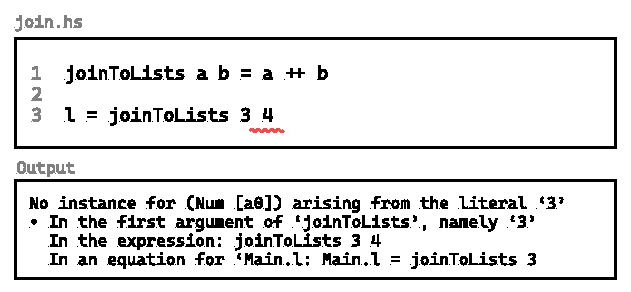
\includegraphics[width=\linewidth]{TypeErrorExample2}
  \caption{
    \label{fig:type-error-example-2}
  In this example, similar to the previous example, with the only change being the function's name, the programmer intended to write the function to concatenate two lists but apply the function with 2 integer values. However, in the type error, only the first argument is reported as an offending code; the second argument is spared. This means changing the literal \texttt{3} to \texttt{[3]} is not enough to resolve the type error; it only updates to a slightly different error message.
    }
\end{figure}

\subsection{Missing Links In Type Errors}
\label{subsec:missing-link}

One of the most frustrating aspects of type errors is that they do not show the complete steps of how to arrive at the conclusion. In the example in Fig \ref{fig:type-error-example-3}  programmer may intend to compare to a char literal \texttt{' '} instead of string literal \texttt{" "}. However, there are multiple clues that contribute to the logic of this conclusion: the definition of the function \texttt{trimWhiteSpace}, the application of \texttt{filter isSpace a}, the definition of \texttt{isSpace}, and even the type signature of \texttt{filter} are all needed to understand how the error happens. In addition, these clauses need to be read in logical order (not necessarily ordered by their appearance in the source) to support natural comprehension. 


\begin{figure}[hbt]
  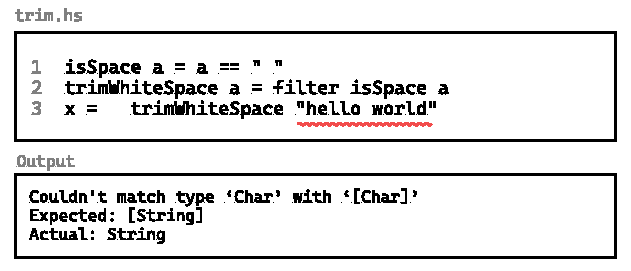
\includegraphics[width=\linewidth]{TypeErrorExample3}
  \caption{
    \label{fig:type-error-example-3}
  In this example, the programmer may intend to compare to a char literal \texttt{' '} instead of a string literal \texttt{" "}. However, the type error ignores all the important clues of how this error is inferred. 
    }
\end{figure}


\subsection{The Use of Obscure Language}

One that often upsets beginners is that type errors are often full of technical jargon or awkwardly phrased sentences. We have seen the common error such as \texttt{No instance for (Num a) arising from the literal `3'} which is a terrible way to convey that a char-typed value is used at a place where a number type is required. "Error messages appear to take the form of natural language, yet are as difficult to read as source code". This bad design of type error messages is not unique to Haskell. In fact, this is often the common behavior in all programming languages and has been shown in many studies \cite{Barik2017-gy, Tirronen2015-nr, Prather2017-dg}. Many studies have sought to improve programmers' ability to solve errors by rephrasing the error message in a way that supports understanding \cite{Becker2016-kc, Barik2014-ib} all show positive results.


\section{The Open Challenges Of Making Good Type Errors}

One major issue stemming from the promises of statically typed languages is the complexity of the systems and tools that safeguard the type-checking process. Ordinarily, this complexity is hidden away from the users. However, most compiler tools fail in usability when encountering incorrectly typed programs. Type errors can be notoriously difficult to understand and use, particularly for newcomers to programming or when using a language that is particularly strict about types. Type errors are often believed to be a major contributor to static typing's reputation of being a high barrier to entry. I believe it is important to understand the root of the challenges of using type errors in order to address them. To achieve that, I believe it is useful to put type errors in proper context, more specifically, comparing them with other classes of programming errors (parsing errors, runtime errors). 

\subsection{Types Are As Complex As Runtime Values}
A major issue that many programming language designers often overlook (or neglect) is that the types are very complex. In languages that implement dependent types, types share the same capability as programs despite the fact that types are only computed at compile time. Even in programming languages that are not as featureful as dependently typed ones, type checking is shown to be non-terminating and Turing complete~\cite{Wells1999-ob}. For instance, in TypeScript, the feature `conditional type' allows programmers to write fully working computations \cite{fig:ts-conditional}. This gives rise to the challenge of explaining the complex reasoning when this type-level computation misbehaves, as we will see, with an unfair lack of debugging facilities.


\begin{figure}[hbt]
  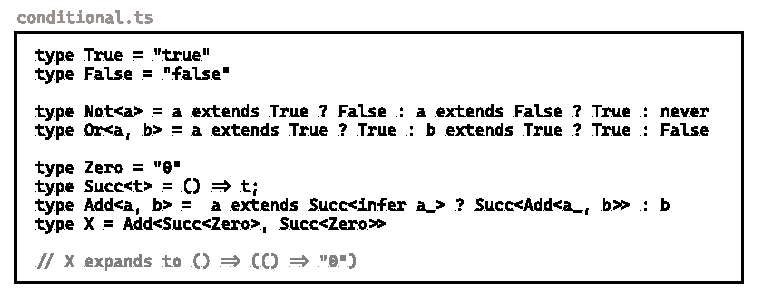
\includegraphics[width=\linewidth]{Conditional}
  \caption{
    \label{fig:ts-conditional}
   TypeScript introduced a feature called conditional types, allowing programmers to write complex logic at the type level. This will allow type annotation to be as complex as the program it describes.
    }
\end{figure}

\subsection{Clues For Type Checking May Be Implicit}
Understanding how types are assigned in a program becomes more challenging when the programming language uses type inference. Type inference \cite{Damas1982-sc},  also known as implicit typing, is a technique that allows programmers to omit the ritual of writing type annotations altogether, and the type checker will infer the most general types (principal types) for each expression. Even for languages that don't employ implicit typing, some typing rules are hidden from programmers.

For example, different programming language has their own rules of what can be compared in an equality check, typically by using a \texttt{==} operator. In programming languages that have a record data type, programmers are burdened with considering adding an extra field or removing a filed still type correct or not \ref{fig:row-polymophism}, often taking into account the language-specific rules such as covariance, contravariance, and subsumption.

\begin{figure}[hbt]
  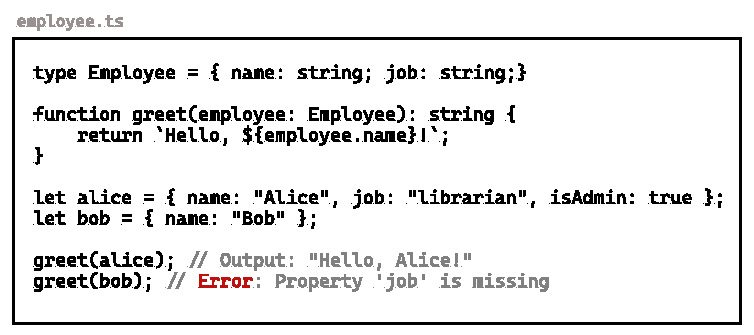
\includegraphics[width=\linewidth]{RowPolymorphism.pdf}
  \caption{
    \label{fig:row-polymophism}
   In many languages support row-polymophism, programmers enjoy more freedom in the fields of a data collection,  depending on situation,  extra fields or missing fields are allowed. However, the rule of subsumptions (which type can substitute another type) is also obscured.
    }
\end{figure}


\subsection{Lack of tool support}
Debugging programming errors has been an essential part of programming since the beginning of computing, dating back as early as 1949 \cite{Campbell-Kelly1992-rn}. However, support for debugging type errors is unfairly lacking compared to runtime error debugging tools. 

To begin with, the simplest and most reliable approach is to insert \texttt{print} statement. "The most effective debugging tool is careful thought coupled with judiciously placed print statements", as put by computing pioneer Brian W. Kernighan \cite{Kernighan1978-xs}.  In addition, breakpoint debugging is a very common debugging method that has been integrated into almost all programming IDEs \ref{fig:breakpoint}. Moreover, research in supporting error debugging has been very active. ZStep94 \cite{Lieberman1995-lg} extends the idea of breakpoint debugging without the need to add any breakpoint, allowing programmers to see all the historical values assumed by an expression. It also allows programmers to incrementally navigate forward and backward in execution history. WhyLine \cite{Ko2009-uf} is a Java program IDE that embraces the idea of a natural programming environment \cite{Myers2004-fy}. It allows programmers to ask questions in the program about why certain behavior happens or does not happen. 

However the develoment type debugging has frozen in time, as most programming languages and develoment environments present type error the same manner as FORTAN and ALGO. Recent years, a few languages, such as Elm and Rust, have taking actions to improve type errors. Unfortunately, the changes they have made are superficial.

\begin{figure}[hbt]
  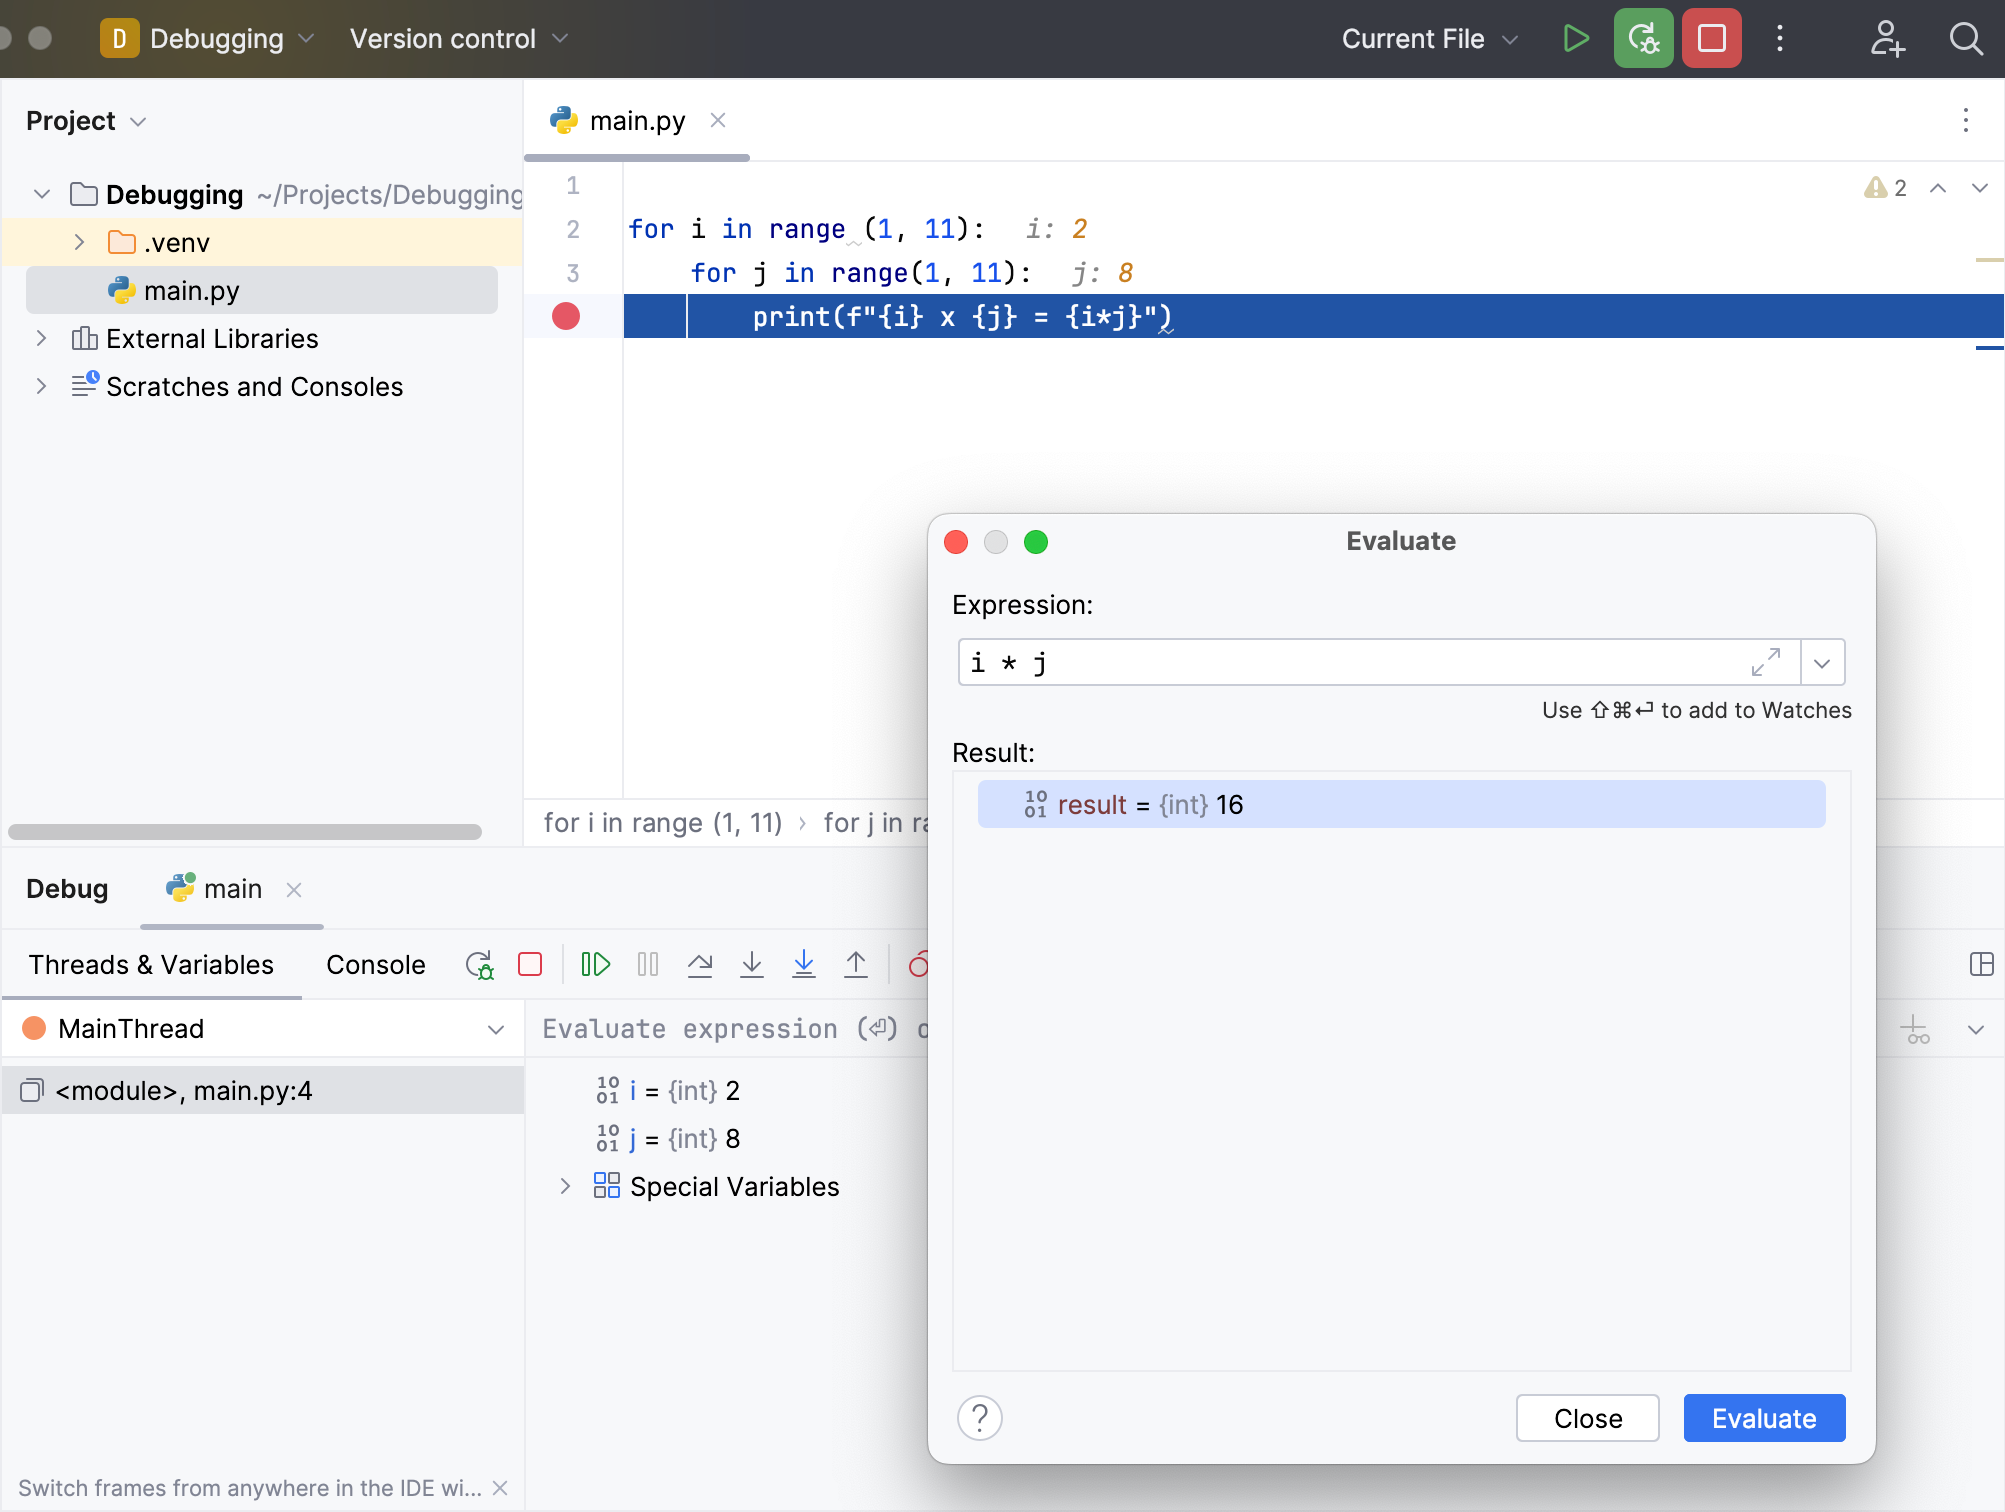
\includegraphics[width=\linewidth]{BreakPoint}
  \caption{
    \label{fig:breakpoint}
    Debugging a Python program using a breakpoint debugger and expression evaluation in PyCharm.
    }
\end{figure}

% \begin{figure}[hbt]
%   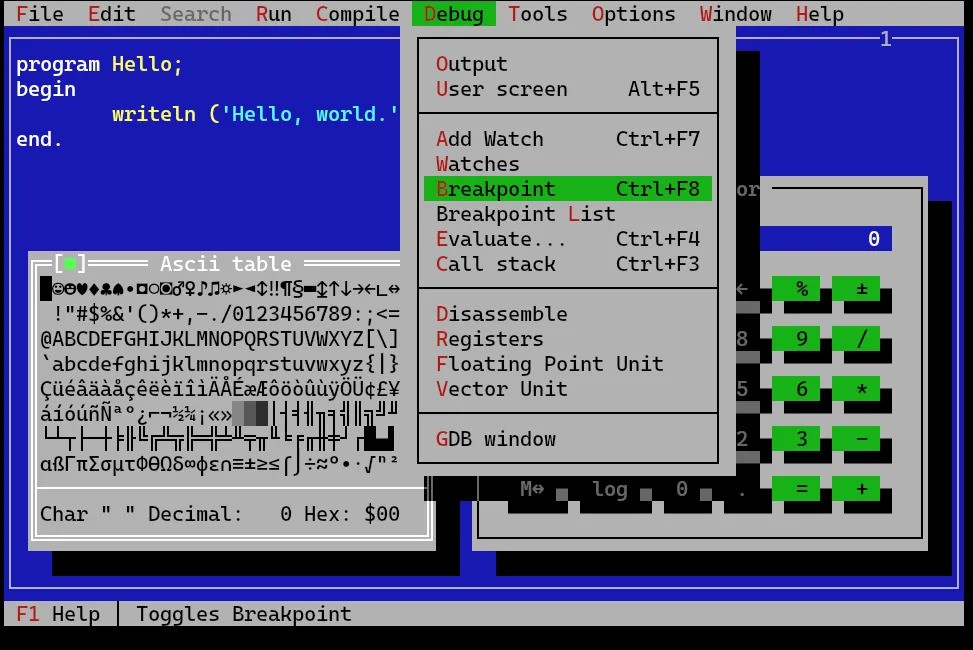
\includegraphics[width=\linewidth]{FreePascal.jpg}
%   \caption{
%     Run time debugging using break point in the Free Pascal interactive development environment in a command line window
%     }
% \end{figure}

% \begin{figure}[hbt]
%   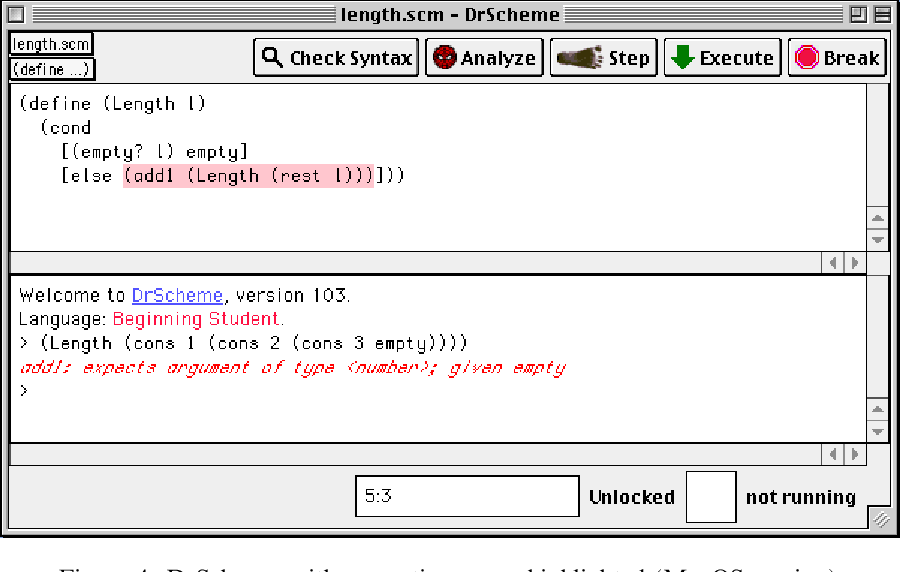
\includegraphics[width=\linewidth]{DrScheme}
%   \caption{
%     Dr Scheme, an interactive development environment for the Scheme language, highlights a runtime error
%     }
% \end{figure}

My research is motivated by the inherent difficulties in debugging type errors and the dormant development of improving type errors using modern graphical capabilities and HCI techniques.

\section{Research Aim}

\subsection{Aim 1. Provide Programmers With The Comprehensive Knowledge Needed to Understand and Resolve Type Errors.}

To date, there is no unified representation of type errors. Most contemporary compiler tools represent type error by providing three pieces of information: a location where the type checking failed, an expected type, and the actually encountered type. As we showed in the previous section, this formulation is far from being helpful and practical. Thus, we question what is needed to explain a type error comprehensively. We try to address this question by carefully examining the limitations of existing systems (\ref{sec:symptoms}) and the thought process of how programmers solve type errors in real life.

\subsubsection{Objective 1.1 To Encompass Multiple Potential Causes Of A Type Error}
One important focus of my work is to address the bias in traditional type errors (Section \ref{subsec:bias}). In this, we need to inform programmers that there exist more than one possible cause of a type error, just as there are multiple ways to resolve such error. To achieve this, the dimension of potential causes is the key information that needs to be clearly communicated. In addition, each potential cause comprises a few key questions: What is the offending code, and what are the resulting type assignments for each expression after the offending code is fixed?

\subsubsection{Objective 1.2 To Accurately Report Relevant Locations Contributing to Type Errors.}
Traditional tools are limited to reporting a single location for type errors, which many researchers have criticized. This leads to programmers often not being able to find a resolution at the reported location and are forced to expand their search without further guidance. We aim to improve this by reporting accurate locations relevant to the type of error.

\subsubsection{Objective 1.3 To Give Reasons And Support Human Understanding}
Type error does not end with a location in the source code. Programmers can still struggle to resolve a type error even after reaching the exact location of the culprits. Failing to understand the logical explanation is equally frustrating than erroneous locations. Internally, type errors can be caused by mismatched types, unfulfilled type class constraints, or trying to construct infinite types. Externally, type errors can be caused by typos, outdated type annotation, incomplete implementation, too few or too many arguments in a function application, etc. Helping programmers find the cause or provide an accurate inference of what is the cause of the type error.


\subsection{Aim 2. Support Programmers To Type Errors Through Interactive Modern Programming Environments.}

We aim to integrate rich type error data into a modern, visual programming environment and workflow that allows programmers to work more efficiently with strongly typed languages. When humans are put in the middle, more information does not equal better comprehension. With enriched data representation, we want to deliver type errors to better support programmers’ comprehension and the chance for a successful resolution.

\subsubsection{Objective 2.1 Communicate The Key Concepts Of Type Errors Effectively Using Modern Programming Tools}

The concepts of type errors are traditionally displayed as text. These concepts include error locations, explanations of causes, and type signatures. We explore more intuitive techniques and media to communicate these concepts and facilitate better comprehension. For instance, using inline highlit to mark the locations directly in the source code provides better usability than printing the lines of interest in the terminal window.

\subsubsection{Objective 2.2 Use Interactive Tools for Investigating and Resolving Type Errors.}

To avoid presenting overwhelming information, we explore different techniques of interactively exploring the type errors. These techniques aim to divide the type error into smaller units that can still be assigned meaning and provide a means for programmers to incrementally triangulate the potential root cause in the source code. This objective also involves providing situation-aware debugging information, meaning that the error message should provide varying levels of detail in the debugging information based on the context of the type of error and the programmer's personal preference.


\section{Contributions}

\subsection{A categorization of type errors based on the structure of the evidence of a type error}

In order to illustrate the challenges of providing a comprehensive explanation of type errors, we divide the type errors into 3 categories. This categorization is based on how it is normally understood from a human debugging perspective. We will give more formal definitions of these categories in Chapter \ref{chap:haskell-type-checking}. It should be made clear that these categories are not mutually exclusive, a multi-witness type error can also be a multi-step type error at the same time.  

A \textbf{multi-step type error} is a type error that involves a chain of logical inferences based on the evidence of the type error. A typical multi-step type error is shown in the example (Fig \ref{fig:multi-step-example}). In the example, the chains of inference are the assignment of a (Line 1), the equivalence of a (Line 1 and Line 2), the assignment of b (Line 2), and the equivalence of b (Line 2 and Line 3). Removing any one of the chains will resolve the conflict. An important challenge with multi-step type errors is to convey this chain of inference relation to the relevant location. 

\begin{figure}[hbt]
  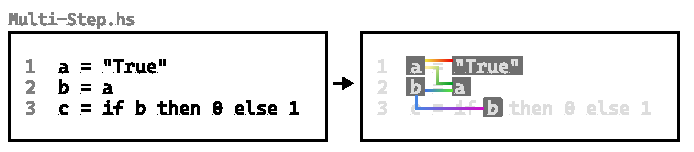
\includegraphics[width=\linewidth]{Multi-Step}
  \caption{
    \label{fig:multi-step-example}
    Illustration of a multi-step type error in Haskell.  The potential issues in the definition of \texttt{a}, \texttt{b}, or the conditional expression of variable \texttt{b}. It can be clearly see a ``chain'' of reasoning formed in order to explain the type error. }
\end{figure}

A \textbf{multi-witness type error} is a type error that involves multiple pieces of evidence supporting the same potential type assignments.  A typical multi-step type error is shown in the example (Fig \ref{fig:multi-witness-example}). In the example, multiple evidence (lines 3,4,5) support that a has the type \texttt{Int -> String}. On the other hand, a single piece of evidence (line 2) shows that a has the type \texttt{Int -> Char}. The challenge of presenting multi-witness type errors is to clearly show the opposing sides and the number of witnesses of each side. 

\begin{figure}[hbt]
  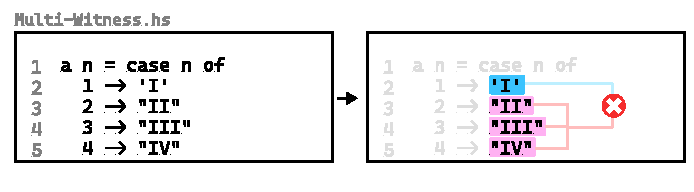
\includegraphics[width=\linewidth]{Multi-Witness}
  \caption{
    \label{fig:multi-witness-example}
    Analysis of a multi-witness type error, where the \texttt{case} expression could be interpreted as type \texttt{Char} or \texttt{String}. This scenario showcases a type disagreement with  witnesses (in color pink) against one witness (in color blue). It is not hard to see that the difference in number play an important role here as the char literal \texttt{'I'} on line 2 is more likely be a typo.
    }
\end{figure}

A \textbf{multi-party type error} is a type error that involves more than two typing possibilities.  A typical multi-step type error is shown in the example (Fig \ref{fig:multi-party-example}). In the example, the expression \texttt{d} can not be assigned a type because 3 pieces of evidence on line 1 suggest 3 potential types for \texttt{d}. In practice, a multi-party type error is considered less intuitive and harder to explain properly. The most prominent task is to break down the type error into multiple simpler forms of type errors. 



\begin{figure}[hbt]
  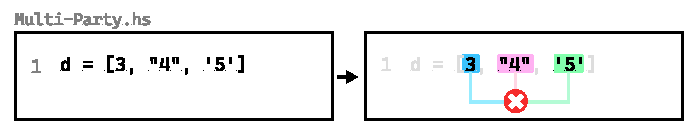
\includegraphics[width=\linewidth]{Multi-Party}
  \caption{
    \label{fig:multi-party-example}
    Analysis of a multi-party type error regarding the list \texttt{d}, which could alternately be typed as \texttt{[Int]}, \texttt{[String]}, or \texttt{[Char]}. The conflict is depicted as a disagreement among three parties (Right). Unlike the previous two examples, this error cannot be fixed by a single location. }
\end{figure}

With this classification, we contributed three systems—Chameleon, Goanna, and GeckoGraph—each focusing on one or two unique challenges of type error debugging.

\subsection{Explaining Multi-Step Type Errors Through Chain-Of-Thought Visualization}

\subsubsection{Technical Contribution - Chameleon}
We contribute Chameleon, an interactive type error debugging tool for Haskell. Internally, Chameleon computes all relevant locations that contribute to the type of error. Via a set of iteratively designed interfaces, Chameleon preserves the two alternatives of the type error and the supporting evidence for each. Chameleon provides a unique debugging interface that allows interactive explore the chain of reasoning in a multiple-step type error. In this interace, programmers see a pair of locations at a time, they are also shown how the two locations are logically related. This allows programmers to develop a panorama view of the type error interactively. 

\subsubsection{An evaluation on the effect of error slicing and chain of thought visualizations}
We contributed a series of studies on the effects of debugging with visual representation of types and interactive exploration of type errors. Our inquiry is whether there is a difference between using traditional tools and enhanced type error debugging tools like Chameleon. 

\subsection{Iterate potential causes of multi-witness and multi-party errors}

\subsubsection{Technical Contribution -- Goanna}
We contribute Goanna, a type error debugging tool for Haskell. 
Similar to Chameleon, Goanna provides a comprehensive set of relevant locations that contribute to the type error and provides alternatives to the type error. More importantly,  Goanna presents a type error by dividing it into a list of potential causes and their respective fixes. With Goanna, Haskell programmers can resolve type errors by exploring a list of potential root causes of errors. We also contribute a set of heuristics that rank potential causes and eliminate unhelpful ones. 

\subsubsection{An evaluation on accuracy, conciseness, and performance of MCS-based type debugging and our heuristics}

We evaluated Goanna's effectiveness using 86 diverse Haskell programs from online discourse, demonstrating its ability to accurately identify and resolve type errors. We are interested in finding out through a few empirical analyses how Goanna compares existing Haskell compilers in explaining the type error correctly, succinctly, and efficiently.


\subsection{Visualizing Types}

\subsubsection{Technical Contribution -- GeckoGraph}

We contribute GeckoGraph, a graphic notation for Haskell types. GeckoGraph describes the same information as type signatures but uses colors, shapes, and symbols to make certain structures easy to identify at a glance. GeckoGraph is designed to use visual elements to improve the understanding of type-level concepts, such as type classes, parametric type variables, and high-rank types. When used to compare two types, GeckoGraph helps clarify differences visually. It makes errors like too few or too many arguments in applications and unmet type class constraints obvious.

\subsubsection{An evaluation on how programmers use graphic type notation}

We conducted a large-scale study on the effectiveness of using GeckoGraph to perform a series of Haskell tasks. We concluded that with GeckoGraph, programmers are more likely to succeed in programming tasks involving polymorphic types. The difference is more significant among programmers with less experience.

% \section{Research Method}

% \subsection{Human-centered programming language studies}

% One important decision that shape a lot of my work is employing human-centered research methods with our novel programming language systems. The adopting of human-centered methods happens at every stage of the projects: prototyping, development and evaluation. Although the using of these methods are not new at all, but they certainly are not the most polular choices in programming language studies.

% The motive of such decision is that it is impossible to understand what are the good qualities of type errors without observing how human use type errors to gain understanding. 


% The downside of study programming language is iterative design is very hard. programming tasks involves complex inputs and outputs, and it is very hard to study an incomplete system without a fully working systems. For instance, if we are to study the effect of type errors, it is most effective to have a system that can recognize type-correct program from ill-typed one. It is hard to evaluate with a mock-up or wizard of oz style fake outputs to study users' interaction.  To address this limitations, we have a few ideas implemented in our research:

% A minimal but practical set of language 
% Design for human from start



\section{Thesis outline}

The thesis can be divided into two parts. The first part (Chapters 1 and 2) surveys the vivid panorama of type systems and programming languages. The purpose of these chapters is to situate the body of work in later chapters and to introduce the proper definitions and terminologies used in this thesis.  The second part (Chapters 4, 5, 6, and 7) delves into three pieces of work, each targeting a unique problem in type error debugging.


\subsection{Chapter 2}
This chapter provides some technical background, including the traditional methods of Haskell type checking, error slicing, and interactive debugging. Following this direction, we continue to discuss the tools and techniques in constraint satisfiability analysis that we use in later chapters to improve type error reporting. Last, we revisit the categorization of type errors and provide a new way to define their meanings with the help of definitions we explored in Chapter 2.


\subsection{Chapter 3}
This chapter introduces the work related to Chameleon and our study on its effect on debugging type errors. This chapter starts with an introduction of our motivation, succinctly summarised in three characteristics of bad-type error messages. We then introduce the key features of Chamaleon, using the example of hypothetical programmers combating Haskell-type errors, luckily with the help of Chameleon. We introduce the system design and iterative prototyping methods used to develop Chameleon. Lastly, we present our experiments on Chameleon's effect on solving type errors compared to traditional compiler tools. 


\subsection{Chapter 4}

In Chapter 5 we discuss our work: the Goanna type debugger and our evalution on its key aspects (accuracy, conciseness and performance). We first report some common limitations of traditional compiler error messages. We then go on to showcase some novel features of Goanna, including suggesting fixes, ranking causes by their likelihood, type error isolation, and cross-module type error debugging.  Next, we discuss the implementation of Goanna and our heuristics for ranking potential causes and removing unhelpful suggestions. Last, we show our empirical study of Goanna's accuracy, conciseness, and performance using a collection of real-world type errors in Haskell code. 

\subsection{Chapter 5}

In this chapter, we discuss our work on visualizing type annotations. In this, we showed GeckoGraph, a visual notation for Haskell type. We also present our empirical study on how programmers use polymorphic types and the effect of GeckoGraph. We start by presenting some usability challenges in using polymorphic types. We then describe the design goal of GeckoGraph and how it can be constructed from a textual type annotation using a few construction rules. We then show our large-scale study on the effect of using visual type annotations in programming and solving type errors. 


\subsection{Chapter 6}

In the last chapter, we reiterate our contributions with more remarks on their contexts. We discuss a few directions for future work. This includes the direction in future tool development, as well as future research opportunities. Lastly, in closing words, we return to the map field of programming language and the vast uncharted area of the future of programming. 